\section{Findings - reveal correlation of speed and mobile data access}

With the speed estimates, we show and explain our findings on correlations of user mobility and mobile data access patterns in this session. We start with the correlation of speed and average mobile data access volume. Then we revealed the relation of speed and average gaps between consecutive mobile data access. In the last, we show the correlation between speed and the apps that are used to generate mobile data traffic.

\subsection{experiment settings}

Our algorithm can only estimate speed when a user has visited more than 3 towers, so only 13 million records out of 58 million records have a speed estimate. In our experiments, to balance the accuracy of speed estimates and the volume of mobile data access records that have qualified speed estimates, we set the threshold of both distance ratio $d_{ratio}$ and duration ratio $\Delta t_{ratio}$ at 0.6. After the filtering, we have around 1 million records out of total 13 million records that meet both criterion. Fig.~\ref{fig:speed_hist} shows the histogram of speed estimates.

\begin{figure}[h]
    \centering
    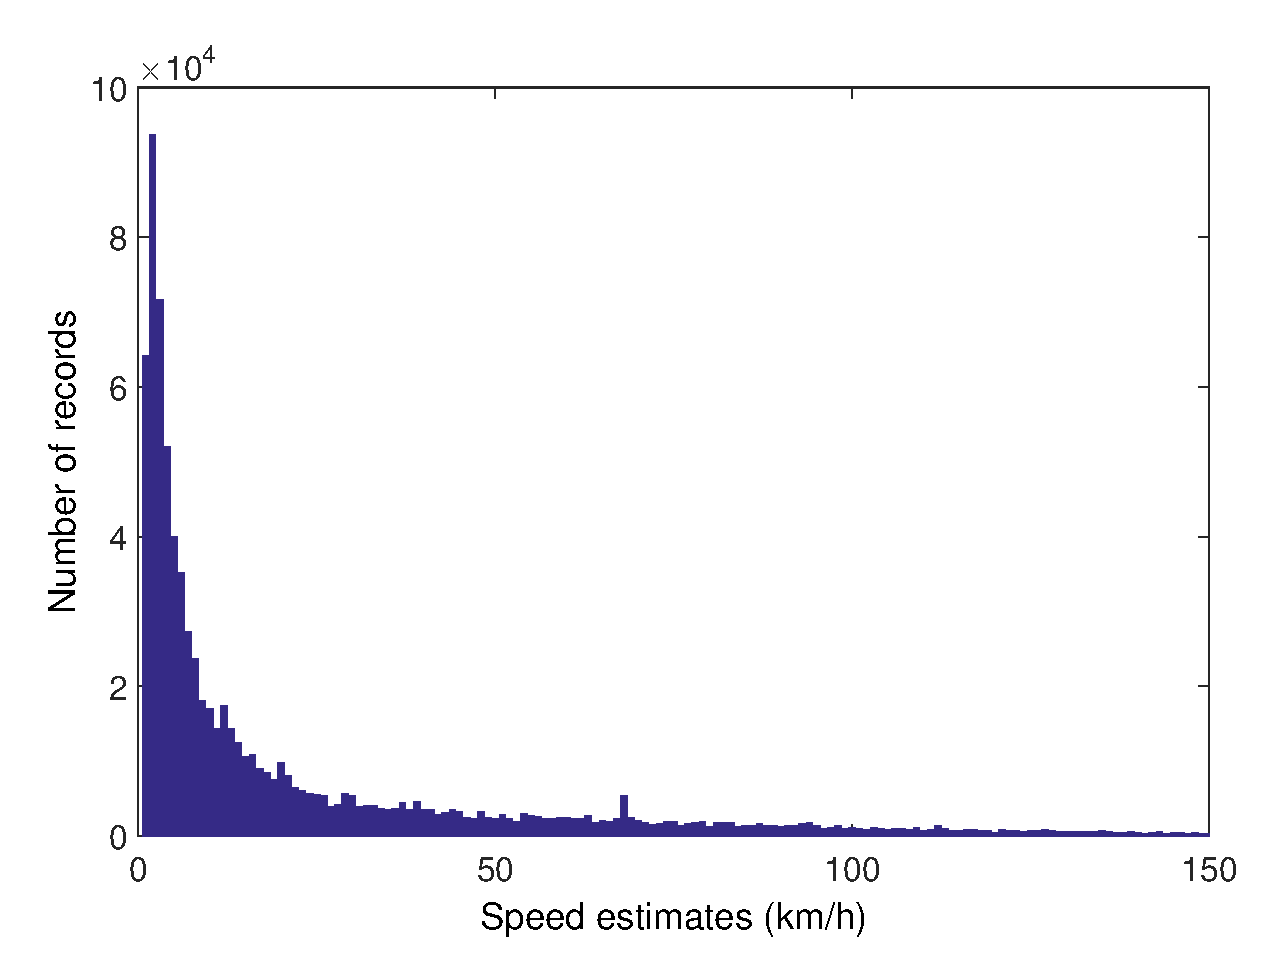
\includegraphics[width=\linewidth]{./figures/speed_hist.pdf}
    \caption{Histogram of speed estimates.}
    \label{fig:speed_hist}
\end{figure}

In the following experiments, we only show results in the speed range of 0 km/h to 100 km/h, since there is very few records have speed estimates above 100 km/h to gain any meaningful insights. 

\subsection{correlation of speed and mobile data access volume}

\begin{figure}[h]
    \centering
    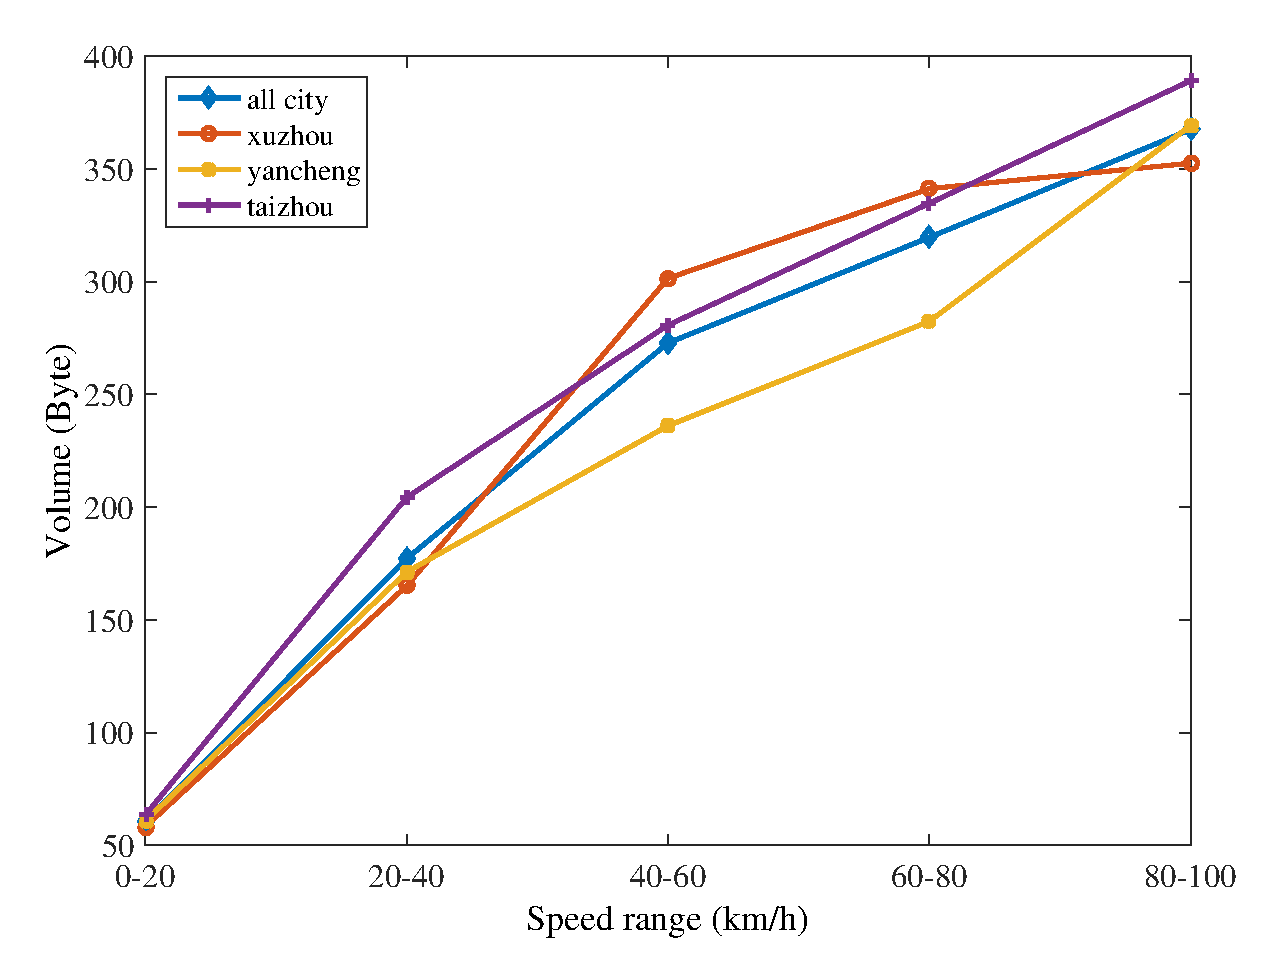
\includegraphics[width=\linewidth]{./figures/speed_vol.pdf}
    \caption{Correlation of access volume and user speed.}
    \label{fig:speed_vol}
\end{figure}

Fig.~\ref{fig:vol_speed} shows the results of the correlation of speed and average mobile data access volume per user per second. We show data from all three cities combined and each city respectively. The figure shows a clear trend that users are more active in access mobile data as the speed increases.
A user with speed estimates of 80-100 km/h could reach a average data volume of 6 times of a low speed user. And this trend holds for all the cities. Note that this does not suggest lower speed users do not access online contents less frequently since they have more sources to reach online contents than high speed users, i.e. WIFI, Ethernet. Previous work ~\cite{yang2015characterizing} reaches similar results while using number of towers visited by user as indicator of user mobility.

\subsection{speed and mobile data access frequency}

\begin{figure}[h]
    \centering
    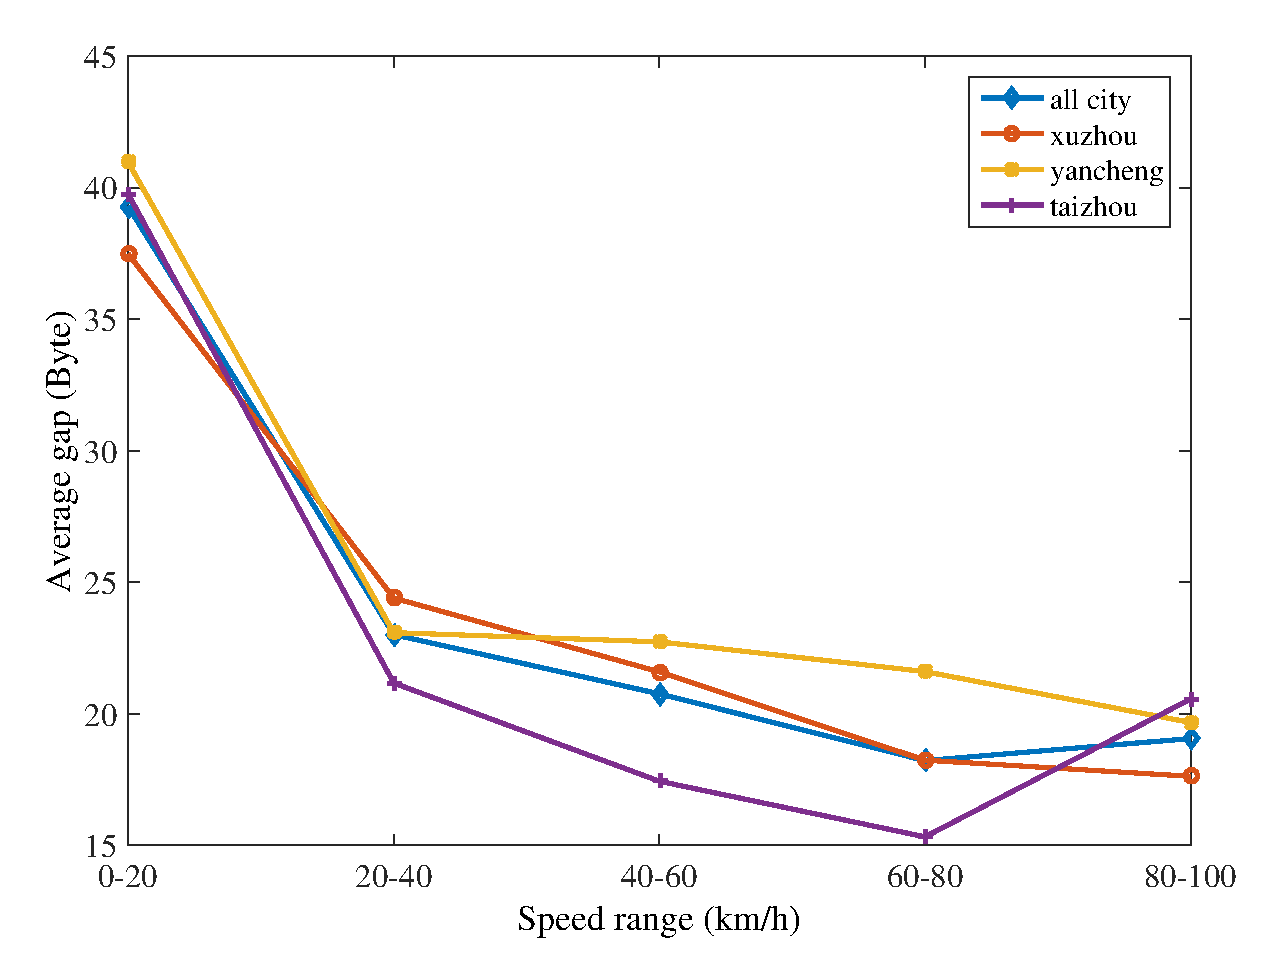
\includegraphics[width=\linewidth]{./figures/speed_gap.pdf}
    \caption{Correlation of time interval between consecutive data access and user speed.}
    \label{fig:speed_gap}
\end{figure}

Fig.~\ref{fig:speed_gap} shows the results of the correlation of speed and time intervals between consecutive mobile data access records. The decrease in the time interval as speed increases suggest that high speed user access mobile data more frequently than low speed users. A user with speed estimate of 80-100 km/h access mobile data almost 2 times more frequently than a user with speed estimates of 0-20 km/h on average. The trend holds for all three cities except that there is an odd point at 80-100 km/h for the city 'taizhou', which may caused by the lacking of available amount of data.

\subsection{speed and mobile data access pattern}

\begin{figure*}[ht]
    \centering
    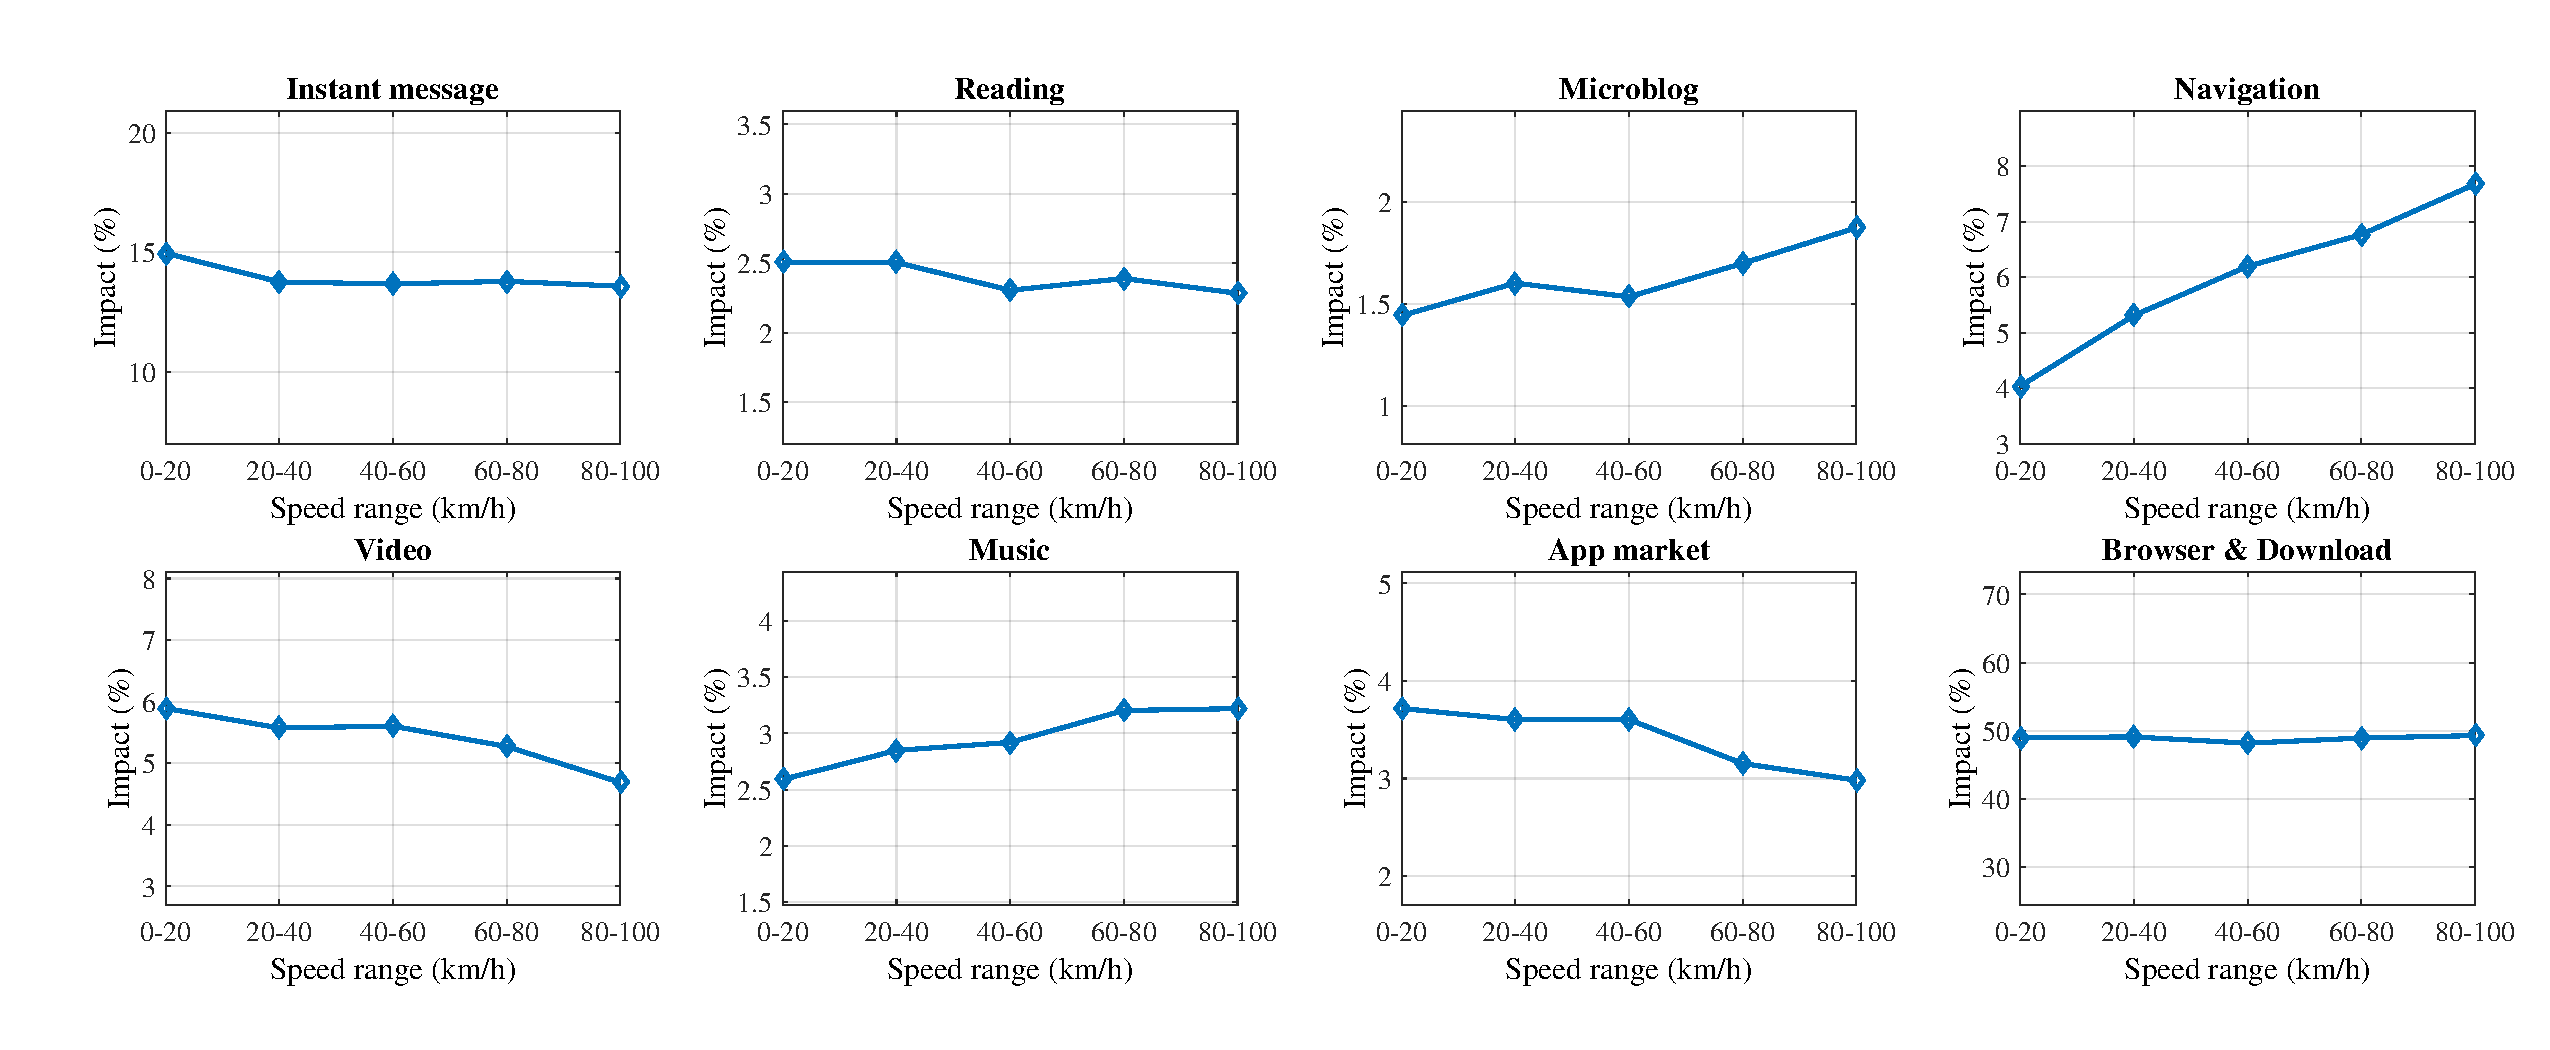
\includegraphics[width=\linewidth]{./figures/speed_appcat.pdf}
    \caption{Correlation of access pattern and user speed.}
    \label{fig:speed_appcat}
\end{figure*}

In this section we study how the impact of various app categories change for different speed range. The impact is defined as the mobile data access of one category versus all categories. As we shown in Table~\ref{table:appcat} that the volume of data for each category is not even, among all 19 categories, we only interested in the app categories that contribute most to the total mobile data access volume. Note that apps in other1 and other2 are those can hardly classify to any other 17 categories. Since they do not share common properties, thus we do not take them into consideration. We select the top 8 app categories with most impact on mobile data access and show their impact changes in fig.~\ref{fig:speed_appcat}. 

Among the top 8 categories, microblog, navigation, music shows an clear trend of increasing as speed increases. The impact of navigation has the most steady increase due to the increased needs for such apps when driving. The impact almost doubles for users with speed estimates of 80-100 km/h compared to users with speed estimates of 0-20 km/h. Instant message, video and app market shows a trend of decreasing as speed increases. The reason could be the users are cost sensitive and dose not want to spend mobile data on large app downloading or video streaming. Brower \& downloading and reading shows a quite stable impact that does not changes a lot as speed increases.
